\documentclass[unicode,12pt,aspectratio=169]{beamer}

\graphicspath{{../fig/}}
%%%%%%%%%%%%%%%%%%%%%%%%%%%
\usepackage{luatexja}% 日本語したい
\usepackage[haranoaji,no-math,deluxe,expert,nfssonly,match,scale=1.0]{luatexja-preset}
\renewcommand{\kanjifamilydefault}{\gtdefault}% 既定をゴシック体に

\usepackage{amssymb,amsmath,ascmac}

\usepackage{multirow}
\usepackage{lltjext}

\usepackage{siunitx}
\usepackage{physics}
\AtBeginDocument{\RenewCommandCopy\qty\SI}
\ExplSyntaxOn
\msg_redirect_name:nnn { siunitx } { physics-pkg } { none }
\ExplSyntaxOff

\usepackage{animate}
\usepackage{svg}
\usepackage{xparse}
%%%%%%%%%%%%%%%%%%%%%%%
\usepackage{tikz}
\usetikzlibrary{shapes,arrows}
\usetikzlibrary{positioning}
\usetikzlibrary{angles,quotes}
\usetikzlibrary{math, calc}
\usetikzlibrary{decorations.markings,decorations.pathmorphing}
%% define fancy arrow. \tikzfancyarrow[<option>]{<text>}. ex: \tikzfancyarrow[fill=red!5]{hoge}
\tikzset{arrowstyle/.style n args={2}{inner ysep=0.1ex, inner xsep=0.5em, minimum height=2em, draw=#2, fill=black!20, font=\sffamily\bfseries, single arrow, single arrow head extend=0.4em, #1,}}
\NewDocumentCommand{\tikzfancyarrow}{O{fill=black!20} O{none}  m}{
\tikz[baseline=-0.5ex]\node [arrowstyle={#1}{#2}] {#3 \mathstrut};}

%目次スライド
% \AtBeginSection[]{
%   \frame{\tableofcontents[currentsection]}
% }
%アペンディックスのページ番号除去
\newcommand{\backupbegin}{
\newcounter{framenumberappendix}
\setcounter{framenumberappendix}{\value{framenumber}}
}
\newcommand{\backupend}{
\addtocounter{framenumberappendix}{-\value{framenumber}}
\addtocounter{framenumber}{\value{framenumberappendix}} 
}

%%%%%%%%%%%  theme  %%%%%%%%%%%
% \usetheme{Copenhagen}
\usetheme{metropolis}
% \usetheme{CambridgeUS}
% \usetheme{Berlin}

%%%%%%%%%%%  inner theme  %%%%%%%%%%%
% \useinnertheme{default}

% %%%%%%%%%%%  outer theme  %%%%%%%%%%%
\useoutertheme{default}
% \useoutertheme{infolines}

%%%%%%%%%%%  color theme  %%%%%%%%%%%
%\usecolortheme{structure}

%%%%%%%%%%%  font theme  %%%%%%%%%%%
\usefonttheme{professionalfonts}
%\usefonttheme{default}

%%%%%%%%%%%  degree of transparency  %%%%%%%%%%%
%\setbeamercovered{transparent=30}

%%%%%%%%%%%  numbering  %%%%%%%%%%%
% \setbeamertemplate{numbered}
\setbeamertemplate{navigation symbols}{}
\setbeamertemplate{footline}[frame number]

%%%%%%%%%%%%%%%%%%%%%%%%%%%%%%%%%%%
% \setbeamertemplate{items}[default]
\setbeamertemplate{enumerate item}[default]

% セクション名だけをTOCに出力
\setcounter{tocdepth}{1}



\title{第五章 レオロジー理解のための基礎的事項 II}
\subtitle{～簡単な微積分とそれによる力とポテンシャル～}
\date{}

\begin{document}
\maketitle

%% 目次 (必要なければ省略)
\begin{frame}
\frametitle{Outline}
\tableofcontents
\end{frame}

\begin{frame}
	\frametitle{この章でのお話}
	具体的なレオロジーの議論に入る前に、もう少しだけ、これからの議論に必要となる数学と物理の基礎的な事項について確認していきましょう。
	
	ここでは、前章よりは少し難しい話になり、高校から大学レベルのお話をすることになります。
	具体的な事項を以下に列記しました。
	\begin{itemize}
		\item レオロジーで扱う関数について
		\begin{itemize}
			\item 指数関数と対数関数について
		\end{itemize} 
		\item 微積分について
		\begin{itemize}
			\item 微積分の見直しと簡単な微分方程式
		\end{itemize} 
		\item 物理モデルを物質の物理とつなげるために
		\begin{itemize}
			\item 力、仕事、ポテンシャルと微積分
		\end{itemize} 
	\end{itemize}
\end{frame}


\section{力と仕事を物理モデルで}

\subsection{力、仕事、エネルギー}
\begin{frame}
	\frametitle{力とは}
	\begin{block}{力とは}
		\begin{itemize}
			\item 「物体の状態を変化させる原因となる作用、\\
			その作用の大きさを表す物理量」
			\item \textcolor{red}{単純化した仮想的な状態（高校の物理）}として、\\
			「慣性系」で「保存力」を考える。 
			\begin{itemize}
				\item 力の定義は、結構面倒。
				\item「慣性系とか保存力って何？」の話はしない
				\item 現時点では\textcolor{red}{摩擦や熱を考えていない。}
			\end{itemize}
		\end{itemize}
	\end{block}
	% \begin{alertblock}{$F=ma$ の意味}
	% 	\begin{itemize}
	% 		\item $m$ という「質量（変化の受け難さ）」を持った物体に、
	% 		\item $F$ という「力」を作用すると、
	% 		\item $a$ という「加速度」で運動（状態変化）する。
	% 	\end{itemize}
	% \end{alertblock}
\end{frame}

\begin{frame}
	\frametitle{仕事とエネルギー}
	\begin{columns}[c, onlytextwidth]
		\column{.48\linewidth}
			\begin{block}{仕事とは}
				\begin{itemize}
					\item 質点に力を作用し移動すること
					\item 仕事は作用させた力 $F$ と\\移動した距離 $s$ の積
				\end{itemize}
				\begin{center}
					
\includegraphics[width=.8\textwidth]{work.png}
				\end{center}
			\end{block}
		\column{.48\linewidth}
			\begin{block}<2->{エネルギーとは}
				\begin{itemize}
					\item 仕事をする能力のこと
					\item 物体や空間は状態変化に伴い\\エネルギーを蓄える
					\item 仕事とエネルギーの次元は同一
				\end{itemize}
			\end{block}
	\end{columns}
	\begin{block}<3>{仕事の次元と単位}
		\begin{itemize}
			\item 次元：[仕事] = [力][距離] = [$ML^2T^{-2}$]、単位：ジュール J
		\end{itemize}
	\end{block}
\end{frame}

\subsection{ポテンシャルと力と微積分}
\begin{frame}
	\frametitle{仕事とポテンシャル}
		\begin{columns}[c, onlytextwidth]
			\column{.6\linewidth}
				\begin{block}{ポテンシャルとは}
			\begin{itemize}
				\item \alert{基準の状態}を定めて
				\begin{itemize}
					\item その着目する状態にするために
					\item 物体あるいは空間に加えた\alert{仕事の量}
				\end{itemize}
				\item 逆に言えば
				\begin{itemize}
					\item ある状態から基準の状態に戻るまでに
					\item \alert{外に取り出せるエネルギーの量}
				\end{itemize}
				\item 力が「\textcolor{red}{保存力}」の場合は
				\item ポテンシャルが「位置のみの関数の\\\textcolor{red}{状態量}」となる
			\end{itemize}
		\end{block}
			\column{.38\linewidth}
				\begin{block}{保存力の定義：}
					\begin{itemize}
						\item 仕事が経路によらない
					\end{itemize}
				\end{block}

				\begin{block}{状態量：}
					\begin{itemize}
						\item 系の状態だけで、\\一意に決まる物理量
					\end{itemize}
				\end{block}
		\end{columns}
\end{frame}

\begin{frame}
	\frametitle{ポテンシャルと力}
	\centering
	\begin{minipage}{.9\textwidth}
		\begin{columns}[c, onlytextwidth]
		\column{.6\linewidth}
			\only<1>{\begin{block}{ポテンシャル $U(\vb{r})$は}
				\begin{itemize}
					\item 基準の位置 $\vb{r_0}$ から
					\item 位置 $\vb{r}$ までの
					\item 力 $F(\vb{r})$ の積分であり、
					\item 位置ベクトル$\vb{r}$の関数
				\end{itemize}

				\vspace{-8mm}
				\begin{align*}
					W(\vb{r}) = \int_{\vb{r_0}}^{\vb{r}} F(\vb{r}) \dd \vb{r} = -U(\vb{r})
				\end{align*}
			\end{block}}
			
			\only<2>{\begin{block}{力 $F(\vb{r})$は}
				\begin{itemize}
					\item 任意の位置$\vb{r}$において
					\item ポテンシャル$U(\vb{r})$ を
					\item $\vb{r}$で微分すれば
				\end{itemize}
					\begin{align*}
						\dv{\vb{r}} U(\vb{r}) = -F(\vb{r})
					\end{align*}
			\end{block}}
			
			\only<3>{
				\begin{alertblock}{バネの場合は}
				\begin{itemize}
					\item 力は $F(x)=-kx$
					\item ポテンシャル $U(x)$ は
					\begin{align*}
						U(x) 
						&= -\int_0^x F(x') \dd x' \\
						&= \dfrac{1}{2}kx^2
					\end{align*}
				\end{itemize}
			\end{alertblock}
			}
		\column{.4\linewidth}
			\begin{center}
				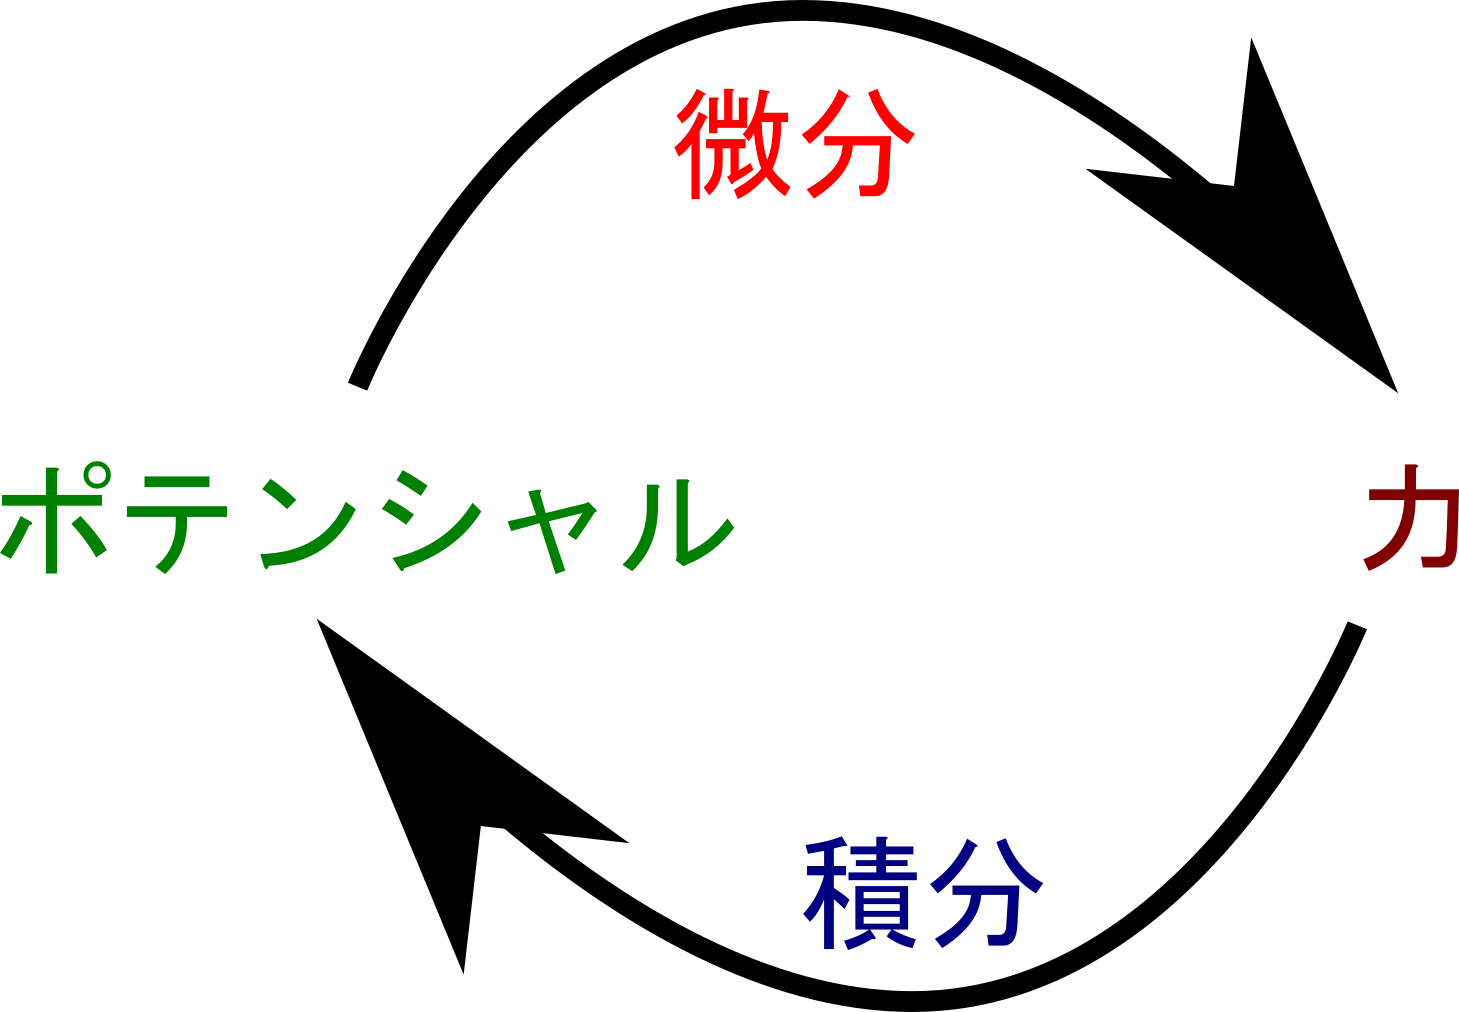
\includegraphics[width=\textwidth]{potential_power.png}

				ポテンシャルと力は\\互いに入れ子
			\end{center}
	\end{columns}
	\end{minipage}
	
\end{frame}

\subsection{摩擦と熱}
\begin{frame}
	\frametitle{摩擦について}
		\begin{columns}[c, onlytextwidth]
			\column{.5\linewidth}
				\begin{block}{摩擦と熱とエネルギー}
					\begin{itemize}
						\item 摩擦力は非保存力
							\begin{itemize}
								\item ポテンシャルは状態量ではなく\\経路に依存
							\end{itemize}
						\item<2-> 内部の粒子の摩擦により、
							\begin{itemize}
								\item 粒子の運動エネルギーが増加し\\系全体の温度が上昇
								\item 非断熱系では、熱エネルギー\\として外界に散逸。
							\end{itemize}
						\item<3> \alert{非保存力も含めれば、\\系全体のエネルギーは保存}
					\end{itemize}
				\end{block}
			\column{.45\linewidth}
				\begin{center}
					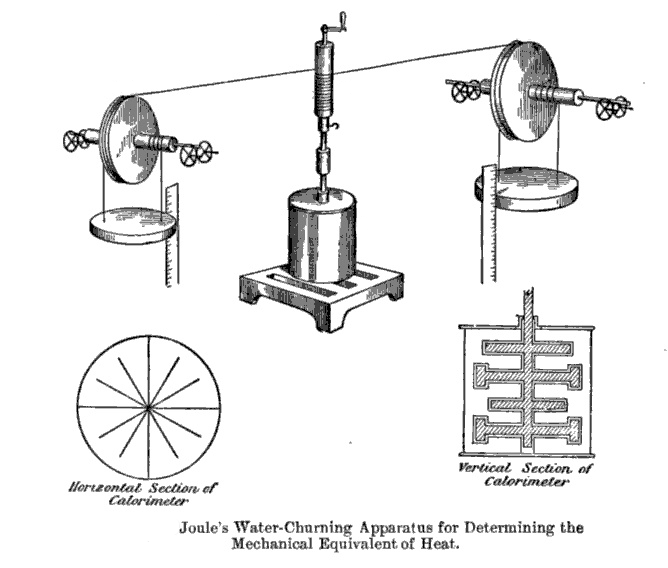
\includegraphics[width=\textwidth]{thermal_eng.png}
					ジュールの試験
				\end{center}
		\end{columns}
\end{frame}


% \section{この章のまとめ}
\begin{frame}
	\frametitle{まとめ}
	% この章では、以下に示したような、ちょっとだけ小難しくなった数学と物理の事項を学びました。
		\begin{boxnote}
			\begin{itemize}
				\item 数学的な事項について
					\begin{itemize}
						\item 指数関数とその逆関数である対数関数の確認
						\item 微分が「瞬間的な振る舞い」、積分が「全体の量を把握」
						\item 簡単な微分方程式から「指数関数的な応答」を理解
					\end{itemize}
				\item 物理に関する事項として
					\begin{itemize}
						% \item 「次元解析」や「無次元量」について
						\item 力、仕事、エネルギー、ポテンシャルを確認し
						\item それら相互の関係と微積分について
						\item 摩擦と熱についても
					\end{itemize}
			\end{itemize}
		\end{boxnote}
\end{frame}

% \appendix
% \backupbegin

% \section{数学関連のメモ}
% \subsection{指数の性質について}
% \begin{frame}
% 	\frametitle{指数の性質（整数への拡張）}
% 	\begin{columns}[T, onlytextwidth]
% 		\column{.5\linewidth}
% 			\begin{block}{指数が 0 の場合は？: $a^0$}
% 				\vspace{-5mm}
% 				\begin{align*}
% 				&a^n \times a^0 =a^{(n+0)} = a^n \\
% 				\therefore \;\;&a^0 = 1
% 				\end{align*}
% 			\end{block}
% 			\begin{block}{負数への拡張: \\$a^{-k}$ ($k$ が正の整数)}
% 				\vspace{-5mm}
% 				\begin{align*}
% 					&a^k \times a^{-k} = a^{k+(-k)}=a^0=1 \\
% 					&\; \text{$a^k (\ne 0)$ で両辺を除すと、} \\
% 					&\therefore \; a^{-k} = \dfrac{1}{a^k}
% 				\end{align*}
% 				指数が負 $\Rightarrow$ 指数が正の逆数
% 			\end{block}
% 		\column{.46\linewidth}
% 		\begin{alertblock}{指数同士の割り算}
% 			\begin{itemize}
% 				\item \textcolor{red}{割り算は指数が負}に\\なると考える。
% 				\item 結局、以下のように\\\textcolor{red}{指数の引き算}となる。
% 			\end{itemize}
% 			\begin{align*}
% 				a^n \textcolor{red}{\divisionsymbol  a^m} 
% 					&=a^n \textcolor{red}{\times \dfrac{1}{a^m}} \\
% 					&= a^n \textcolor{red}{\times a^{-m}} \\
% 					&= a^{n + (-m)}
% 			\end{align*}
% 		\end{alertblock}
% 	\end{columns}	
% \end{frame}

% \begin{frame}
% 	\frametitle{指数の性質（有理数への拡張）}
% 		\begin{block}{}
% 			\begin{columns}[T, onlytextwidth]
% 				\column{.48\linewidth}
% 					\begin{itemize}
% 						\item $a^{\frac{1}{n}}$（$n$ は整数）を $n$ 乗\\することを考える。
% 							\begin{equation*}
% 								(a^{\frac{1}{n}})^n=a^{\frac{1}{n} \times n} = a
% 							\end{equation*}
% 						\item すなわち、\\ $a^{\frac{1}{n}}$ の $n$ 乗が $a$
% 					\end{itemize}
% 				\column{.48\linewidth}
% 					\begin{itemize}
% 						% \item 実数 $x$ に対して、
% 						\item $x$ を $n$ 乗（$n$ は正の整数）すると $y$ になるとき、
% 						\begin{itemize}
% 							\item $y$ を「$x$ の $n$ 乗根」
% 							\item $\sqrt[n]{x}$ と表記
% 						\end{itemize}
% 					\end{itemize}
% 			\end{columns}
% 		\end{block}
% 	\begin{alertblock}{指数が分数の場合}
% 		\begin{itemize}
% 			\item 分数の分母となる値を用いて累乗根を表し、
% 			\item 分子はそのべき乗を表すこととなり、
% 			\item 以下のように記述できる。
% 		\end{itemize}
% 		\begin{equation*}
% 		a^{\frac{m}{n}}=\sqrt[n]{a^m}
% 		\end{equation*}
% 	\end{alertblock}
% \end{frame}

% \section{演習問題 1}
% \subsection{「レオロジーで扱う関数について」}
% \begin{frame}
% 	\frametitle{「レオロジーで扱う関数について」}
% 	\small
% 		\begin{itemize}
% 			\item \textcolor<2>{black}{冪}とは、「\fbox{\textcolor<1>{white}{底}}」と呼ばれる正の数の右肩に「\fbox{\textcolor<1>{white}{指数}}」と呼ばれる数を載せた数式表現。
% 			\item 同じ底の累乗同士の掛け算は、\fbox{\textcolor<1>{white}{指数同士の足し算}}となる。
% 			\item 累乗のさらなる累乗は、\fbox{\textcolor<1>{white}{指数同士の掛け算}}となる。
% 			\item 指数同士の割り算は、\fbox{\textcolor<1>{white}{指数の引き算}}となる。
% 			\item 指数が分数の場合、分数の分母となる値が\fbox{\textcolor<1>{white}{累乗根}}を表し、分子はその\fbox{\textcolor<1>{white}{べき乗}}を表す。
% 			\item 物理的な議論では、底に\fbox{\textcolor<1>{white}{ネイピア数}} e を多用。
% 		\end{itemize}
% \end{frame}

% \backupend

\end{document}